\documentclass[11pt]{article}
\usepackage[margin=1in]{geometry}
\usepackage[T1]{fontenc}
\usepackage{times,microtype}
\usepackage{amsmath,amssymb}
\usepackage{booktabs,graphicx,xcolor}
\usepackage[numbers,sort&compress]{natbib}
\usepackage[colorlinks=true,linkcolor=blue!60!black,citecolor=blue!60!black,urlcolor=blue!60!black]{hyperref}
\usepackage[capitalize,noabbrev]{cleveref}

\newcommand{\E}{\mathbb{E}}
\title{\textbf{When Should a Self-Written Skill Branch?}}
\author{Manoj Bajaj \qquad Devin (Cognition AI)}
\date{}

\begin{document}
\maketitle

\begin{abstract}
Feedback can steer a reusable skill toward a common preference, or pull it toward incompatible preferences. A single compromise skill cannot serve both optima when it must act identically for both users; branching cannot help if the agent lacks a cue before acting. We test a writer that hill-climbs on noisy common-item comparisons, forks one steering coefficient into two when estimated cue-specific targets have no acceptable shared coefficient, and rejoins when they agree. Across 64 synthetic streams with 90\%-accurate cues, branching improved first-conflict worst-cohort utility over a learned shared MaxMin baseline by 0.093, but lost 0.312 to a fixed cue-conditioned policy. It used 1.57 live coefficients on average versus two for the fixed policy, while storing an additional feedback window. It never branched on 64 single-hill streams, but also missed all conflicts with weaker cues and fell below MaxMin there. The result supports routing over a cue-blind compromise in this test, not adaptive branching over fixed conditioning.
\end{abstract}

\begin{figure}[!h]
  \centering
  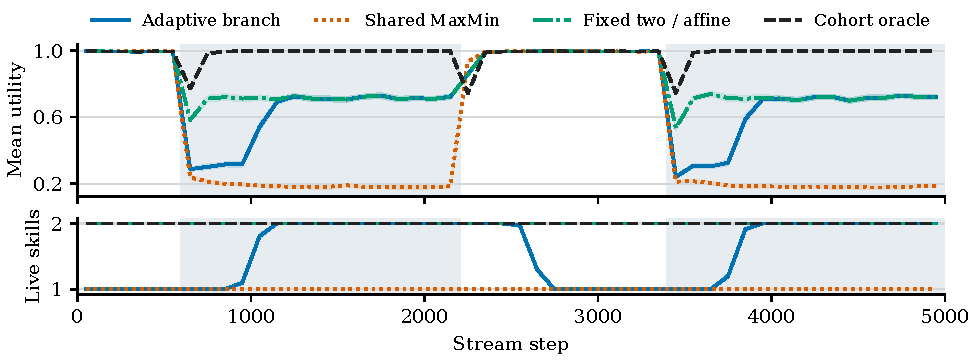
\includegraphics[width=\linewidth]{timeline.pdf}
  \caption{\textbf{Adaptive branching delays specialization and frees a serving slot when preferences agree.}
  Mean utility over arriving requests (top) and live steering coefficients (bottom) in 100-step bins, averaged across 64 routable streams; bands are pointwise 95\% seed intervals.
  Shaded background marks conflict and reversed conflict. Only the oracle sees true cohort labels.}
  \label{fig:timeline}
\end{figure}

\section{Introduction}
\label{sec:intro}
An agent that revises a skill from user feedback can treat each correction as a direction to climb. If the users prefer the same outcome, their feedback can improve a single skill. If they prefer different outcomes on the same request, a better compromise still need not satisfy either user. MaxMin-RLHF formalizes an egalitarian objective for a policy trained on diverse preferences~\citep{chakraborty2024}; a different response is to keep the useful versions apart and choose one using information available when the next request arrives.

Detecting disagreement is not enough. Two feedback streams can look different because they compare different items, because feedback is noisy, or because the users prefer different outcomes. Even when the hills truly differ, the writer cannot benefit from fitting two versions if the executor cannot tell which one to use. Conversely, distinct versions need not be permanent. If the users converge on a shared preference after a revision, the executor could go back to serving one coefficient.

We isolate these issues in a scalar steering task. A fixed executor adds a mutable style coefficient to a task-specific response. An online writer updates the coefficient from noisy comparisons of the same two alternatives conditional on the item, and uses a pre-action cue, not a cohort label, to test whether one coefficient can serve both cue groups. The test first requires credible separation, then clones the serving coefficient; when the same test supports agreement, it collapses the two coefficients. A fixed two-slot control has the identical observation and update rule without waiting for evidence to allocate slots.

With a strong cue, two versions work: the cohort-label oracle scores 0.971 on the first conflict, and fixed cue conditioning scores 0.544, compared with 0.139 for the learned shared MaxMin baseline (\cref{tab:main}). Adaptive branching scores 0.232 and saves live coefficients, but has no total-state advantage here. It also underperforms the shared MaxMin baseline with weaker cues (\cref{tab:cue}). Thus a small online detection rule can decide when to specialize in this fixture, but does not beat a standing cue-conditioned skill.

\section{Problem}
\label{sec:problem}
At step \(t\), an observable item contributes an offset \(b_t\) and an optional preference signal is represented by a binary cue \(c_t\in\{0,1\}\). A latent cohort \(g_t\in\{0,1\}\) defines a preferred offset \(\theta_t\in[-0.9,0.9]\). The simulator scores the action \(a_t=b_t+w_t(c_t)\) by
\begin{equation}
  u_t(a_t) = 1-(a_t-b_t-\theta_t)^2.
  \label{eq:utility}
\end{equation}
A skill is the reusable steering coefficient \(w\in[-1,1]\), not the task offset or the simulator's hidden target. A shared skill ignores the cue; a routed skill selects one of two coefficients. Scores can be negative. The learner never observes its score or \(\theta_t\). The oracle alone knows \(g_t\), and it still has to learn the coefficients.

After acting, the writer receives one noisy comparison on the same item, between \(b_t+h\) and \(b_t-h\), with \(h=0.5\). The simulator generates their utility difference plus independent Gaussian noise with standard deviation \(4h\sigma\), where \(\sigma=0.55\). Dividing by \(4h\) gives the scalar margin \(z_t=\theta_t+\epsilon_t\), \(\epsilon_t\sim\mathcal{N}(0,\sigma^2)\). This is a cardinal comparison, not a binary vote. Because the compared offsets are the same for all users, the data cannot create an apparent preference split solely by showing different alternatives. All methods use exactly one such comparison per step.

\paragraph{One action or one policy?}
In the conflict phases the cohort optima are \(m\) and \(-m\), with \(m=0.9\). For a cue-blind coefficient the largest squared error is \((m+|w|)^2\), minimized at \(w=0\), giving worst-cohort utility \(1-m^2=0.19\) even with known preferences. That is also a bound for randomized cue-blind actions independent of cohort in a stationary phase (\cref{app:math}). It is not a bound on a single policy that uses the cue. With a binary cue, two served coefficients \(w_0,w_1\) are exactly one affine map \(w_0+(w_1-w_0)c\). We therefore distinguish branch \emph{allocation} from representational advantage.

\section{Writing and branching}
\label{sec:method}
\paragraph{Ascent.}
After receiving \(z_t\), update only the served coefficient:
\begin{equation}
 w \leftarrow \mathrm{clip}_{[-1,1]}\{ w+\alpha(z_t-w)\},\qquad \alpha=0.035 .
 \label{eq:ascent}
\end{equation}
The expected update before clipping is half a utility gradient scaled by \(\alpha\). Before a split the update pools all arrivals; after a split it updates one child using \(c_t\). All coefficients start at zero.

\paragraph{Branch criterion.}
For a stationary cue-conditional target mean \(\mu_j=\E[\theta_t\mid c_t=j]\), expected squared loss at coefficient \(w\) exceeds the best cue-specific squared loss by \((w-\mu_j)^2\). We call a write acceptable if that excess is at most \(\delta^2\), with \(\delta=0.32\). One shared coefficient can satisfy both cue groups precisely when \(|\mu_0-\mu_1|\le 2\delta\). This is a check on cue-group regret, not a guarantee on latent cohort utility.

The writer checks this criterion every 32 comparisons using the last \(W=512\) pairs \((c_t,z_t)\). Let \(n_j\) be the count and \(\hat\mu_j\) the mean of cue \(j\) in the window. It checks only when both \(n_j\ge48\). Let \(d=|\hat\mu_0-\hat\mu_1|\) and \(r_j=3\sqrt{\sigma^2+0.9^2}/\sqrt{n_j}\). It applies the next rule after scoring the current request:
\begin{align}
 \text{split if one slot and}\quad
   & d-r_0-r_1>2\delta \quad\text{and}\quad \max(r_0,r_1)\le\delta ;
   \label{eq:split}\\
 \text{rejoin if two slots and}\quad
   & d+r_0+r_1\le 2\delta.
   \label{eq:rejoin}
\end{align}
Under the interval assumptions, \cref{eq:split} says no shared coefficient meets both floors, while each estimated mean lies within its respective floor for all true means in its interval. This is a witness for candidate coefficients, not for the currently served coefficients. Upon splitting, both children inherit the live coefficient and keep learning by \cref{eq:ascent}; on rejoin, their mean initializes the shared coefficient. Otherwise the writer retains its current slot count. The checks are spaced and hysteretic, but their radii are not an anytime-valid test; mixed windows at real changepoints do not estimate a stationary target.

\paragraph{Controls.}
Pooled ascent keeps one coefficient and uses \cref{eq:ascent}. Shared MaxMin also serves one coefficient; it estimates the first and second moments of \(\theta_t\) separately for each cue, then maximizes the lower estimated utility across the two cue groups (\cref{app:math}). This is a quadratic analogue of the single-compromise objective, not a reproduction of MaxMin-RLHF. Fixed two uses \cref{eq:ascent} with two cue-indexed coefficients from step zero; interpreted as an affine cue-conditioned skill it has the exact same predictions and state dimension. The cohort oracle uses the same update but indexes by the hidden cohort. It is a positive control with extra information, not an attainable baseline.

\section{Evaluation}
\label{sec:eval}
\paragraph{Streams and accounting.}
Each run has 5,000 arrivals: 600 on a common initial target, 1,600 with minority cohort B gaining a different target, 1,200 with both cohorts agreeing at a third target, and 1,600 with their conflicting targets reversed. The probability of B changes from 0.02 to 0.30 at the first conflict, rises to 0.55 on agreement, and returns to 0.30 at reversal. The one-hill control retains the same composition shifts and cue accuracy, but everyone has the same target at each step. Cue-strength controls change only the probability of the cue matching the cohort, to 0.65 or 0.50 instead of 0.90. Conditions and methods use matched random draws across seeds 1000--1063. Full generator constants and metric definitions are in \cref{app:protocol}.

All methods do one scalar selection and add at serving time and receive one comparison per request. Pooled ascent stores one mutable scalar, fixed two and the oracle two, and Shared MaxMin stores five including its serving coefficient. Adaptive branching serves one or two but also maintains 512 float64 margins, 512 int8 cues (4,608 payload bytes), two sums, two counts, and a position counter. The ring maintenance is constant per comparison with a constant-size check every 32. Counts exclude Python object overhead for all methods. We match feedback, not memory or write computation. The full run took 8.4 s on an Intel Xeon CPU; model training and external API calls are absent.

\begin{table}[!ht]
\centering
\caption{\textbf{Fixed cue conditioning outperforms adaptive branching in the first conflict.}
Per-cohort and worst-cohort utility over the first conflict and average live serving coefficients over the full routable stream, mean \(\pm\) 95\% seed interval half-width (64 seeds). Higher utility is better. The coefficient column excludes the writer's feedback state; only the oracle can route by cohort.}
\label{tab:main}
\begin{tabular}{lrrrr}
\toprule
Writer & Cohort A \(\uparrow\) & Cohort B \(\uparrow\) & Worst \(\uparrow\) & Live coeff. \\
\midrule
\csname @@input\endcsname table_main.tex
\bottomrule
\end{tabular}
\end{table}

\subsection{Branching beats the compromise, not fixed conditioning}
The cohort oracle's 0.971 worst-cohort utility shows that both targets can be learned when routes are known. Fixed cue conditioning reaches 0.544 using only the noisy cue, versus 0.139 for Shared MaxMin. Adaptive branching improves over Shared MaxMin by \(0.093\) (paired 95\% CI \([0.079,0.108]\)) but trails fixed conditioning by \(0.312\) (paired CI \([-0.319,-0.306]\) for adaptive minus fixed; \cref{tab:main}). Separate behavior earns utility under the observed cue. Delaying its allocation loses enough utility that adaptive branching is still behind fixed conditioning over the full stream, by 0.183 on the same worst-cohort metric (paired CI \([-0.186,-0.180]\)).

Waiting is a functional part of the comparison: during the delay the adaptive learner is a pooled writer serving predominantly cohort A (\cref{fig:timeline}). Cohort B pays substantially more than A for the delay; during the first conflict their mean utilities are 0.232 and 0.757, respectively. Keeping the cheaper serving state on the common hill does not pay for that loss in this setup: the fixed policy's two scalar coefficients cost less total state than the adaptive gate's evidence window. We do not infer that fixed conditioning always wins when slots are costly.

\begin{table}[!ht]
\centering
\caption{\textbf{The gate refuses to branch when cue information is weak, even when preferences conflict.}
First-conflict results on 64 paired seeds; in the one-hill control the same interval has a common target. Utility difference is adaptive minus Shared MaxMin (paired mean \(\pm\) 95\% interval half-width). Split rate is percent of streams with a new split in the interval, with a 95\% Wilson interval. Delay is conditional on observed splits; a blank design cell inherits the base setting.}
\label{tab:cue}
\begin{tabular}{lrrrr}
\toprule
Condition & Cue accuracy & Worst utility \(\Delta\) & Split \% & Delay (steps) \\
\midrule
\csname @@input\endcsname table_cue.tex
\bottomrule
\end{tabular}
\end{table}

\subsection{No pre-action information, no reliable routing}
With uninformative cues, conditioning on the cue does not change the target distribution. With weaker cues, a true difference between latent cohorts does not imply that cue groups differ enough for the specified loss tolerance. In the synthetic conflict with 30\% B traffic, Bayes' rule gives population cue-mean gaps of 1.348, 0.460, and 0 for cue accuracies 0.90, 0.65, and 0.50 respectively. Only the first exceeds \(2\delta=0.64\). The gate's behavior in \cref{tab:cue} is consistent with this ordering; it is not evidence that no useful personalization exists at 0.65. Under either weaker cue, the adaptive writer stays pooled, and its worst-cohort score is below Shared MaxMin. A gate on branch allocation does not by itself make its unsplit policy equitable.

Across the entire one-hill stream, including target and composition changes, none of the 64 replicates produced a split (95\% Wilson interval \(0\%\)--\(5.7\%\)). Thus the gate rejects the shared-hill decoy in this fixture; a false-split rate of exactly zero in the population is not established.

\begin{table}[!ht]
\centering
\caption{\textbf{The writer rejoins and forks again after preferences reverse.}
Adaptive writer on 64 routable seeds. Rates use 95\% Wilson intervals, and delays for successful transitions and prequential utilities use mean \(\pm\) 95\% seed interval half-width. A transition is the first matching slot-count change within a phase. Utility uses every request in that phase.}
\label{tab:transitions}
\begin{tabular}{lrrrrr}
\toprule
Transition & Rate \% & Delay (steps) & A \(\uparrow\) & B \(\uparrow\) & Worst \(\uparrow\) \\
\midrule
\csname @@input\endcsname table_transitions.tex
\bottomrule
\end{tabular}
\end{table}

\subsection{Rejoining is reversible, but not free}
Every routable replicate split after the first change, returned to one coefficient during agreement, and split again after reversal (\cref{tab:transitions}). Agreement utility remained high for both returning cohorts when their new target was common. The second fork required new evidence: the writer keeps no dormant child coefficients and does not restore either old version. This is a test of repeated allocation and adaptation, not a test of retaining old skills after an unrelated edit or of preserving separately callable amendment state once the serving copies are removed.

\section{Related work}
MaxMin-RLHF learns a mixture of preferences and optimizes a single egalitarian policy~\citep{chakraborty2024}. Variational Preference Learning instead conditions policy and reward on inferred user latents~\citep{poddar2024}, and MiCRo estimates a mixture preference model with context-aware routing~\citep{shen2025}. Our synthetic comparison treats the cue as an exogenous, imperfect observation and does not learn user embeddings or a router. Fixed conditioning is the relevant counterexample to a claim that two separate serving artifacts are needed.

Sparse mixtures of experts make parameters selectively active as a function of an input~\citep{shazeer2017}. Voyager builds a library of executable skills by iterating on environment feedback~\citep{wang2023}. The experiment here isolates when to change the number of live steering coefficients in a shared task under repeated preference changes; it does not replace expert routing or demonstrate language-based skill induction.

\section{Conclusion}
One cue-blind skill can be the wrong interface for users who want different outcomes on the same item. In this controlled stream, an automatically written pair of steering coefficients improved worst-cohort utility over a learned shared compromise when a pre-action cue had enough signal. The writer returned to sharing when preferences aligned, and forked again when they reversed. But fixed cue conditioning achieved better utility, and in this scalar setting its extra serving coefficient cost less than keeping a detection window. We found no evidence that adaptive branching is a better default than fixed conditioning.

The comparison assumes cardinal matched feedback, a known noise scale, and a fixed cue. A next test should price preference queries, let cue quality vary, and compare adaptive allocation against a shared conditional adapter at matched writer and serving memory. It should also separate repeated allocation from preservation of independent revision rules after a rejoin. The experiment and seed-level results are in the \href{https://github.com/manojbajaj95/cl/tree/devin/1795681610-self-branching-skills/experiments/self_branching_skills}{code repository}.

\paragraph{AI disclosure.}
Manoj Bajaj originated the hill-climbing, conflicting-feedback, and branching framing. Devin (Cognition AI) developed the experimental design from that framing, verified the cited literature records, implemented and ran the experiments, analyzed the results, and wrote the paper. Idea development was mixed; Devin performed the literature work, experiments, analysis, and writing.

\bibliographystyle{plainnat}
\bibliography{references}

\appendix
\section{Quadratic baselines and the cue test}
\label{app:math}
For a cue-blind randomized action \(W'\) independent of the latent cohort, the maximum of the two group risks is at least their mean:
\[
 \tfrac12 \E[(W'-m)^2+(W'+m)^2]=\E[(W')^2]+m^2\ge m^2 .
\]
The deterministic coefficient zero attains this bound on stationary conflict. This population argument concerns the declared cue-blind class, not estimates from noisy finite streams or policies whose past actions can reveal correlated identities.

Shared MaxMin maintains a clipped exponential average of \(z_t\) for the cue mean \(\hat m_j\), and an exponential average of \(z_t^2-\sigma^2\) for the second moment \(\hat q_j\), both with step size \(\alpha\). Its estimated risk is \(w^2-2\hat m_jw+\hat q_j\). Below both estimated means the maximum risk decreases and above both it increases. Between the two means the optimum is their risk crossing, clipped to the interval between the means; if the means coincide the common mean is optimal. The objective accounts for cue groups' different risk constants, unlike simply averaging the location estimates. The extra moment estimates are noisy in the finite stream; the ideal true-cohort, cue-blind first-conflict utility is 0.19, compared with the learned cue-based comparator's 0.139.

For a stationary window, shifts in the mean of \(\theta_t\mid c_t=j\) do not affect the bounded-range sub-Gaussian proxy \(0.9^2\), and independent Gaussian noise adds \(\sigma^2\). Hence the heuristic radii use the corresponding standard scale divided by \(\sqrt{n_j}\); we do not claim sequential error control. For the merge condition, all feasible cue means lie in the corresponding estimated intervals. Their total envelope has diameter at most \(2\delta\) when \cref{eq:rejoin} holds and \(r_j\le\delta\) for both cues. The balanced sample counts here typically make each radius smaller than \(\delta\), but the code checks only the gap bound for rejoin: even when one radius is larger, the bound certifies that for every simultaneous pair of true means there exists a shared coefficient, not that the inherited mean is it.

\section{Reproduction and metrics}
\label{app:protocol}
The three item offsets \(-0.4,0,0.4\) are sampled independently and uniformly. The routable, weak-cue, and hidden streams all use targets \((0,0)\), \((0.9,-0.9)\), \((0.3,0.3)\), and \((-0.9,0.9)\) for cohorts A and B in successive phases; the one-hill condition uses \((0.9,0.9)\) in the second phase and \((-0.9,-0.9)\) in the fourth. Cohorts and cues are simulated binary random variables. The same random draws generate items, feedback noise, group arrivals, and cue flips across competing methods. The writer sees each fresh item and cue before action and receives feedback afterward; phase boundaries, future signals, and true utility scores are not passed to it.

We first compute a stream's cohort utility as the arithmetic mean over its requests in the phase, then take the minimum for the worst-cohort score, and then average across independent seeds. For phases with no requests from one cohort, we omit that cohort from the minimum; all first-conflict and later result rows contain both cohorts. Interval half-widths are Student \(t\) intervals over per-seed statistics, or over within-seed differences for comparisons. Latency is the number of requests from the regime's first item to the first serving decision with the new slot count. Timing intervals condition on a transition, and reported rates include failures. Phase-level means include all waiting and recovery steps. The timeline uses pooled request utility to show transient changes rather than estimating a worst from short, sometimes highly imbalanced bins.

\noindent Reproduce with Python 3.10, NumPy, SciPy, and Matplotlib:
\begin{verbatim}
OPENBLAS_NUM_THREADS=1 python3 experiments/self_branching_skills/run.py
python3 papers/self-branching-skills/plot.py
\end{verbatim}
The first command writes \texttt{seed\_metrics.csv} and \texttt{results.json}; the second generates the vector plot and numerical tables directly from those summaries.
\end{document}
